\chapter{Cơ sở lý thuyết} \label{chap:theory}
    \section{Cấu tạo Quadcopter}
    	\subsection{Bộ khung}
Các phần chính của bộ khung Quadcopter được tóm tắt trong bảng sau:
\begin{tabular}{|c|c|c|}
\hline 
Số lượng & Tên & Kích thước \\ 
\hline 
1 & Bộ điều khiển trung tâm & 155mm \\ 
\hline 
4 & Khung & 330mm \\ 
\hline 
2 & Càng hạ/cất cánh & 220mm \\ 
\hline 
\end{tabular}
\begin{itemize}

\item Bộ điều khiển trung tậm được tạo từ hai tấm vật liệu carbon gắn chặt với nhau và khung Quadcopter. Bộ điều khiển sử dụng chương trình Adrupilot để kiểm soát bay. Ngoài ra bên trong bộ điều khiển còn chứa dây nguồn,… Pin Li-polymer được đặt ở dưới cùng bộ điều khiển để tạo sự ổn định khi bay. 

\item Khung Quadcopter được tạo thành từ các thanh Carbon rỗng. Các thanh này được gắn chặt với bộ điều khiển thông qua các miếng cao su để giảm chấn khi động cơ hoạt động. Bốn thanh Carbon được đặt cách đều nhau. Các động cơ cũng được đặt trên một tấm vật liệu Carbon và gắn chặt với khung bằng ốc vít.

\item Càng Quadcopter cũng được tạo từ các thanh Carbon rỗng. Phần tiếp xúc với trung tậm điều khiển được kẹp giữa hai tấm Carbon để chắc chắn hơn. Phần dưới cùng của càng sẽ tiếp xúc với mặt đất. Nó cho phép Quad-Rotor cất cánh ổn định hơn từ mặt đất.
\end{itemize}
\newpage
       \begin{figure}[h!]
	        	\begin{center}
	        		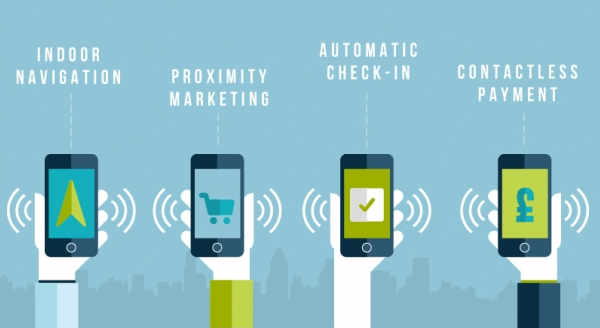
\includegraphics[scale=0.8]{images/retail.png}
	        		\caption{Một Quadcopter}
	        	\end{center}
        \end{figure}
        
    	\subsection{Linh kiện điện tử}
Các linh kiện điển tử sử dụng được tóm tắt qua bảng sau:
\begin{tabular}{|c|c|c|}
\hline 
Số lượng & Tên & Trọng lượng \\ 
\hline 
4 & Bộ điều tốc & 32g \\ 
\hline 
4 & Động cơ không chổi than & 55g \\ 
\hline 
1 & Pin Li-Po & 250g \\ 
\hline 
4 & Phích cắm & 1g \\ 
\hline 
1 & Bộ chuyển đổi 4 ra 1 & 3g \\ 
\hline 
1 & Bộ chuyển đổi điện áp & 3g \\ 
\hline 
1 & AdruPilot Mega 2.5 & 31g \\ 
\hline 
1 & Bộ thu tín hiệu & 9.4g \\ 
\hline 
\end{tabular} 

\begin{itemize}
\item Bộ điều tốc được sử dụng được thiết kế riêng cho động cơ có nhiều Rotor. Mỗi bộ điều tốc nặng 32 gam với kích thước 55mmx26mmx11.6mm (rộng, dài, cao). Bộ điều tốc cung cấp năng lượng cho Motor và kiểm soát tốc độ quay của Rotor. Bộ điều tốc này cũng có chức năng giảm điện áp khi Quadcopter hoạt động ở công suất thấp.

\item Các động cơ được sử dụng là động cơ không chổi than. Mỗi động cơ nặng 55gam (có thể lên tới 800gam tùy vào cánh quạt sử dụng) và có kích thước 27.5mm x 28mm (dài, cao).

\item Pin được sử dụng là pin Li-Po. Nó có điện áp 11.1V và dung lượng pin là 3300mAH. Dung lượng pin càng lớn thì thời gian sử dụng càng nhiều. Do ta đang sử dụng 4 motor nên ta phải dùng pin có năng lượng đủ lớn. Tuy nhiên nếu pin có dung lượng càng lớn thì kích thước và trọng lượng càng tăng. Trong Quadcopter này, ta dùng pin nặng 250gam và có kích thước 43mm x 130mm x 13mm (rộng, dài, cao). Quad-Rotor có thể bay trong vòng 10 – 15 phút với loại pin Li-po này.

\item Các phích cắm được hàn với bộ điều tốc để nối với pin qua lỗ cắm. Nó có thể cho dòng điện có cường độ 40A chạy qua. Ta cũng có thể dễ dàng cắm, rút phích vào/ra lỗ cắm.

\item Bộ chuyển đổi gồm 4 lỗ cắm ra 1 phích cắm. Phích cắm của bộ điều tốc sẽ cắm vào 4 lỗ cắm của bộ chuyển đổi. Phích cắm của bộ chuyển đổi sẽ nối với pin. Chỉ cần 1 bộ chuyển đổi là có thể cấp năng lượng cho 4 bộ điều tốc từ 1 viên pin.

\item Bộ chuyển đổi điện áp có đầu ra là 6 cổng cung cấp điện áp 5.3V và dòng điện 2.25 A. Ta sử dụng bộ chuyển đổi điện áp để cấp nguồn cho ArduPilot Mega. Bộ chuyển đổi chấp nhận nguồn vào lên đến 18V và 90A.

\item ArduPilot Mega 2.5 là một trình điểu khiển hệ thống mã nguồn mở. Phiên bản Ardupilot này có thiết kế PnP, không cần phải lập trình. Tuy nhiên, nó cũng cho phép người dùng lập trình bằng phần mềm Arduino. Chức năng của thiết bị này là biến các phương tiện như xe, thuyền, máy bay thành các phương tiện không người lái.

\item Ta sử dụng bộ thu tín hiệu 8 kênh có tần số 2.4GHz. Nó được kết nối với vệ tinh. AR 8000 hoạt động trên tần số vô tuyến, nó có thể thấy được sự thay đổi của tín hiệu ngoài môi trường. Tín hiệu từ bộ thu sẽ được xử lý bằng phần mềm Spektrum để tạo thành “hình ảnh” sinh động nhất của tín hiệu vô tuyến. Sử dụng tần số 2.4GHz sẽ giúp tín hiệu được truyền tải liên tục, không bị nhiễu bởi các tần số khác. Sau khi kết nối bộ thu - phát tín hiệu thì bộ thu – phát sẽ chỉ kết nối với nhau nên nó không bị các tín hiệu khác làm nhiễu.
        \end{itemize}
    \section{Nguyên lý hoạt động}
    Một Quadcopter gồm 4 động cơ cánh quạt gắn với nhau. Khi động cơ quay, nó sẽ tạo ra lực nâng theo phương thẳng đứng.Cánh quạt quay càng nhanh thì lực nâng càng lớn và ngược lại. Vì thế, Quadcopter có thế bay lên cao hoặc hạ xuống thấp nhờ vào sự thay đổi tốc độ quay của các cánh quạt. Để Quad-rotor bay được thì tổng lực nâng tạo ra bởi 4 động cơ phải bằng hoặc lớn hơn lực hấp dẫn của Quadcopter.  
    Quadcopter có thể di chuyển theo phương ngang bằng cách thay đổi lực nâng của các cặp cánh quạt.    		Nếu tất cả các Rotors quay theo chiều kim đồng hồ, Quadcopter sẽ bị mất kiểm soát do phản lực của momen xoắn. Để tránh trường hợp trên thì ta sẽ cho cặp cánh phía trước (front) và cặp cánh phía sau (back) quay ngược chiều kim đồng hồ, trong khi đó cặp cánh bên phải (right) và bên trái (left) lại quay cùng chiều kim đồng hồ để triệt tiêu các momen xoắn.   
        \subsection{Hệ quy chiếu}
Quadcopter được mô hình hóa theo hệ tọa độ tham chiếu Trái Đất Phẳng. Hệ toạ độ tham chiếu Trái Đất Phẳng bỏ qua lực ly tâm và gia tốc Coriolis.
Khung tham chiếu gồm các trục tọa độ (x, y, z) là hệ thống các trục đơn giản được dùng để xác định số lượng hoặc độ lớn. Hệ trục này có thể được gắn vào thân của vật hoặc Trái Đất. Trong trường hợp này, các trục của vật (xb,yb,zb) đang quay với trọng tâm là Quad-Rotor và các trục Trái Đất (xe, ye, ze) được biểu diễn như hình.                     
        \subsection{Mô hình động lực học}
        Nguyên lý hoạt động chính của mô hình này hoạt động dựa trên sự chuyển động của các dòng khí do cánh máy bay tạo ra và sự điều chỉnh vận tốc quay của cánh quạt sẽ làm thay đổi hướng bay của Quadcopter.\\
        Để mô tả chuyển động của Quadcopter ta cần 2 hệ quy chiếu:
        \begin{itemize}
        \item e1 hệ quy chiếu Trái Đất.
        \item eB hệ quy chiếu khung Quadcopter.
        \end{itemize}
        \\
        Sự định hướng Quadcopter được biểu thị bởi 3 góc Euler qua ma trận xoay R(1)
        \\
        Lực sinh ra của các rotors:
        \\
        Khi đó lực nâng cho cả khung máy bay là:
        \\
        Phương trình mô tả gia tốc Quadcopter:
        \\
        Phương trình quan hệ giữa ma trận quán tính, momen quay M và momen quay hồi chuyển:
        \\
        Ta có momen quay hồi chuyển phụ thuộc vào các yếu tố vận tốc xoay với u1 = T, u2, u3, u4 lần lượt là các đơn vị momen quay các chuyển động roll, pitch, yaw hay vận tốc quay uT=(u1, u2, u3, u4) và vận tốc góc wi máy bay sẽ được g(u) = w1 + w2 - w3 - w4 (5)
        \\
        Kết hợp (5) với (3) và (4) ta có phương trình động lực học: (6) 
        \subsection{Mô hình tính toán khí động học}
        Việc tính toán khí động học mô tả các tác động khi quay của cánh quạt trong không khí. Với các thông số TMT(N) là lực đẩy của cánh quạt, hướng lên, S(m2) là diện tích của cánh quạt, ps (kg/m3) là mật độ không khí
        \\
        Ta có phương trình lực đẩy:
        \\
        TMT = 2psSv12(N)
        \\
        Do lực đẩy TMT = Wp = mg/4 (trọng lượng được mang bởi 1 cánh quạt):
        \\
        Vận tốc dòng khí cho mỗi cánh quạt V1 = \sqrt{(Wp)/(2psS)} (m/s) 
     \section{Bộ điều khiển bay Quadcopter}
     \subsection{Thiết kế bộ điều khiển bay}
            Bộ điều khiển phải đảm bảo rằng Quadcopter phải đáp ứng được các yêu cầu đầu vào một cách chính xác nhất. Một cấu trúc kiểm soát vòng lặp kín được sử dụng trong bộ điều khiển này vì nó sẽ làm giảm sự xáo trộn và thích nghi nhanh với bất kỳ thay đổi nào trong quá trình bay của Quadcopter. Sự phân bố trọng lượng không đều của Quadcopter cũng có thể giải quyết bằng vòng lặp kín.
            \\
            Bộ điều khiển vòng lặp kín phải đảm bảo output phải sát với input. Vòng lặp điều khiển kín là nghịch đảo của động lực Quad-Rotor. Khi biết được động lực của Quad-Rotor, bộ điều khiển sẽ được điều chỉnh và nghịch đảo của động lực Quad-Rotor sẽ được tính. Kết quả tín hiệu điều khiển "U" được đưa vào mô hình để cho ra output mong muốn. 
            \subsection{Nguyên lý hoạt động}
            Bộ điều khiển được xây dựng với các vòng lặp PD. Các vòng lặp PD sẽ có trong các hành vi, độ cao và vị trí của Quad-Rotor để tạo ra tín hiệu điều khiển tương ứng. Quad-Rotor sẽ sử dụng hệ thống điều khiển PD để xác định thời gian phản hồi và giải quyết yêu cầu của nó. Bộ điều khiển PD là một hệ thống phản hồi vòng lặp kín mà nó sẽ dùng output của tín hiệu điều khiển và gửi nó vào tín hiệu input ban đầu. Ta sẽ tính toán được sự khác nhau giữa hai tín hiệu và đưa ra sự điều chỉnh. Trong trường hợp này, vị trí và hướng của Quad-Rotor hiện tại (tín hiệu output) sẽ được gửi đến và so sánh với vị trí và hướng mong muốn (tín hiệu input) để cho phép hệ thống điều chỉnh input và các quá trình tương ứng.
\\
			Tín hiệu sai số được thể hiện bằng.
			\\
			Trong đó, e(t) là tín hiệu sai số, r(t) là tín hiệu input, y(t) là tín hiệu output.
			\begin{itemize}
			\item "Điều khiển tỷ lệ" là thuật ngữ phụ thuộc vào sai số điều khiển. Nó có thể kiểm soát bất cứ phần ổn định nào. Tăng tính cân đối sẽ làm giảm thời gian phản hồi của hệ thống điều khiển. Tuy nhiên, nếu tăng tính cân đối quá cao thì hệ thống sẽ không ổn định. Phương trình cân đối:
\\
Trong đó, u(t) là tín hiệu input trong Quad-Rotor, e(t) là tín hiệu lỗi, kp là gia lượng tỷ lệ.
			\item Điều khiển dẫn xuất là khái niệm output giảm khi các biến quá trình đang tăng. Nó tác động lên tỷ lệ thay đổi lỗi. Tăng điều khiển dẫn xuất sẽ làm cho hệ thống phản hồi mạnh mẽ với các thay đổi của lỗi và tăng tốc độ phản hồi.
			\\
			Trong đó, Kd là hệ số đạo hàm
			\item Để xác định được giá trị của Kp và Kd, ta phải điều chỉnh bộ điều khiển cho đến khi đạt được  phản hồi mong muốn. Ta dùng phương pháp Ziegler-Nichols và thủ công (trong hầu hết các trường hợp) để điều chỉnh các tỷ lệ và giá trị phái sinh. Ngoài ra, ta có thể dùng Simulink để điều chỉnh các giá trị tự động nhưng vẫn đáp ứng được yêu cầu của phản hồi.
			\end{itemize}
			\subsection{Cấu trúc bộ điều khiển}
			Các góc Roll, Pitch, Yaw được điều khiển bởi các vòng lập PD bên trong, trong khi độ cao và vị trí được kiểm soát bởi các vòng lặp PD bên ngoài. Các vòng lặp ngoài sẽ tạo ta các giá trị mong muốn cho vòng lặp bên trong. Ta sẽ tập trung vào từng khối chi tiết trong phần sau.
\\
			\begin{itemize}
			\item Kiểm soát hành vi
			\\Vòng lập bên trong kiểm soát các góc Roll, Pitch và Yaw. Giả sử các trục x,y của Quad-Rotor đối xứng, tức là điều khiển góc Pitch và Roll giống nhau. Góc Pitch giảm khi di chuyển Quad-Rotor về phía trước dọc theo trục X trong khi góc Roll thì di chuyển Quad-Rotor về bên hông.
ROLL: Tín hiệu điều khiển U2 được tạo ra từ roller hoặc được truyền vào thông qua bộ điều khiển PD. Tín hiệu này sẽ điều chỉnh góc Roll của Quad-Rotor.
PITCH: Tín hiệu điều khiển U3 được tạo ra từ pitcher hoặc được truyền vào thông qua bộ điều khiển aPD. Tín hiệu này sẽ điều chỉnh độ cao của Quad-Rotor. Như đã nói ở trên giá trị của P và D của góc Roll và Pitch là như nhau.
YAW: Tín hiệu điều khiển U4 được tạo ra từ yawer hoặc được truyền vào thông qua bộ điều khiển PD. Tín hiệu này sẽ điều khiển góc YAW của Quad-Rotor. Giá trị của các góc Pitch, Roll, Yaw được đo sẽ là giá trị được nạp từ output của mẫu thử.
\\
			\item Kiểm soát độ cao
			\\
			Điều khiển vòng lặp ngoài này sẽ tạo ra một lực đẩy Td để nâng Quad-Rotor lên độ cao mong muốn. Nó được nạp thông qua bộ điều khiển PD. Td sau đó được chuyển đến bộ điều khiển độ cao để bù trừ cho hao hụt do vector của góc Pitch và Roll. Do đó, tín hiệu điều khiển U1 sẽ giữ được độ cao mong muốn của Quad-Rotor mà ngay cả khi góc Roll và Pitch thay đổi. Các khối điều khiển sau sẽ cho thấy vòng điều lặp điều khiển và tín hiệu tương ứng bên trong bộ điều khiển độ cao. Phản hồi nhận được cung cấp độ cao của Quad-Rotor.
\\
			\item Kiểm soát vị trí
			\\
			
		Vòng lặp ngoài này sẽ tính toán các góc roll và pitch để đưa Quad-Rotor đến vị trí X và Y mong muốn. Dữ liệu phản hồi từ mô hình cung cấp giá trị X và Y. Tín hiệu vị trí sau khi tổng hợp được nạp thông qua một bộ điều khiển PD và nó tạo ra các góc Roll và Pitch mong muốn. Như đã đề cập trước đó, output của nó sẽ được nạp vào bộ điều khiển hành vi để tạo ra các tín hiệu điều khiển U2 và U3.
\\
			\item Kiểm soát điện áp của các Rotors
			\\
			Bốn inputs điều khiển được tạo ra bởi các vòng lặp trong và ngoài, nó không nạp trực tiếp vào mô hình Quad-Rotor vì nó là inputs lực đẩy cho bốn động cơ cánh quạt. Các tín hiệu điều khiển U được kết hợp để tạo ra tín hiệu điện áp cho mỗi Rotor. Sự kết hợp này dựa vào lực của Quad-Rotor để hiển thị thông số bay tương ứng. Sự kết hợp này đã được nói ở phần động cơ Rotor và được hiển thị như sơ đồ khối bên dưới. Điện áp đầu ra V sau đó được chuyển thành lực đẩy động cơ của mô hình.
  
			\end{itemize}
            Sau đó, Bluetooth Mesh dùng cơ chế publish-subscribe để các gói tin tới được nơi cần tới. Các địa chỉ unicast được đánh cho các element trong node và được gọi là publish address, còn có multicast address và vitural address bao gồm nhiều element (địa chỉ multicast thường đại diện cho cho một tầng lầu, một phòng,... trong thực tế). Khi có tin mới được gửi đến một địa chỉ publish address, bất kỳ những model nào (element bao gồm nhiều model) trong element và có đăng ký nhận tin (subscribe) ở địa chỉ đó sẽ nhận được tin.
        
            \begin{figure}[h!]
        	    \begin{center}
        		    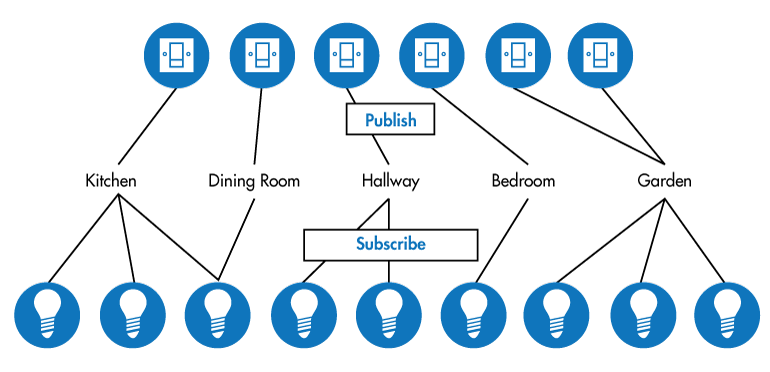
\includegraphics[scale=0.5]{images/mesh-pub-sub.png}
        		    \caption{Sơ đồ của cơ chế publish-subscribe}
        	    \end{center}
            \end{figure}
    \section{Quản lý các phần tử trong mạng}
        \subsection{Tham gia mạng - Provisioning}
            Để một thiết bị mới tham gia vào mạng mesh, cần thực hiện quá trình provisioning. Đây cũng được xem như quá trình bắt tay giữa các thiết bị khi tham gia vào mạng mesh, sau khi hoàn thành quá trình provionsing gồm 5 bước, thiết bị chính thức trở thành node - một thành phần trong mạng. Bluetooth Mesh hỗ trợ hai cách để provision một thiết bị:
            \begin{itemize}
                \item PB-ADV: Sử dụng gói advertising của BLE để tiến hành provisioning bằng cách thay đổi một số trườngww.
                \item PB-GATT: Sử dụng các characteristics của GATT để tiến hành provisioning, chỉ dùng khi thiết bị mới không hỗ trợ advertising hoặc không cho tùy chỉnh gói advertising.
            \end{itemize}

            Ngoài ra, khi thiết bị mới nằm ngoài tầm phủ sóng của provisioner, Bluetooth cũng hỗ trợ provisioning thông qua các node trung gian hoạt động như các relay để gửi các gói tin liên quan provisioning, quá trình này gọi là remote provisioning. Quá trình này có thể không cần thiết trong đa số ứng dụng trong thực tế vì người dùng hoàn toàn có thể mang theo thiết bị provionser như smartphone, sau đó đặt thiết bị mới vừa tầm và tiến hành provisioning. Có thể tham khảo flowchart của quá trình này trong phần \ref{remoteprov}.

            \begin{figure}[h!]
            	\begin{center}
            		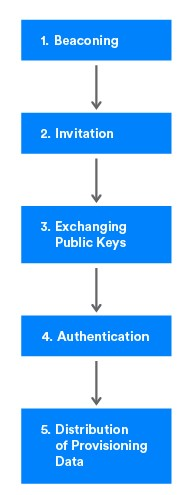
\includegraphics[scale=0.8]{images/mesh-management-fig2.jpg}
            		\caption{Quá trình provisioning gồm 5 bước}
            	\end{center}
            \end{figure}

            Tiếp theo, nhóm sẽ trình bày chi tiết hơn về quá trình provisioning thông qua PB-ADV:
            \begin{itemize}\label{security}
                \item Bước 1 - Beaconing: Khi một thiết bị mới (unprovisioned) muốn gia nhập mạng mesh, thiết bị này sẽ cần Network Key của mạng đó, sau đó tiến hành phát beacon để thông báo sự hiện diện của mình, tùy nhà sản xuất mà quá trình có thể kích hoạt bằng cách nhấn hoặc giữ nút,... Lúc này thiết bị đóng vai trò provisioner - thường sẽ là điện thoại, máy tính bảng có cài ứng dụng đặc biệt - sẽ tiến hành scan thiết bị mới, khi provionser phát hiện được thiết bị mới thì tiến hành bước tiếp theo. Trong đề tài này, nhóm sử dụng node gateway để thực hiện chức năng provisioning vì chưa phát triển được ứng dụng trên điện thoại.
                \item Bước 2 - Invitation: Provisioner sẽ gửi một lời mời, một gói tin Provisioning Invite PDU, đến thiết bị cần provisioning, thiết bị này sẽ đáp lại bằng một gói Provisioning Capabilities PDU, trong đó chứa một số thông tin của nó như số element,... đặc biệt là các input output mà nó hỗ trợ để tiến hành authentication sau này.
                \item Bước 3 - Exchanging Public Keys: Thiết bị mới và provisioner sẽ tiến hành trao đổi public key để dùng cho 2 bước cuối cùng của quá trình provisioning áp dụng giải thuật mã hóa bất đối xứng FIPS P-256 Elliptic Curve Algorithm. Quá trình trao đổi này có thể dùng phương pháp out-of-band để tăng tính bảo mật, out-of-band bao gồm các cách như quét QR code,...
                \item Bước 4 - Authentication: Sau khi biết được các input output mà thiết bị mới hỗ trợ nhờ bước 2, provisioner sẽ gửi yêu cầu sử dụng một trong các phương thức output, chẳng hạn như màn hình LCD hoặc LED, để thể hiện một hoặc nhiều con số (giống với mã PIN khi kết nối Bluetooth giữa 2 điện thoại). Người dùng sẽ quan sát và nhập con số này vào ứng dụng, provionser sẽ gửi và thiết bị mới sẽ kiểm tra để hoàn thành bước này (input/output authentication), hoặc đơn giản hơn là định nghĩa sẵn một dạng mật khẩu nào đó và để 2 bên xác thực bằng mật khẩu này (static authentication). Quá trình kiểm tra này có áp dụng hash để bảo mật.
                \item Bước 5 - Distribution of the Provisioning Data: Provionser sẽ gửi Network Key và cấp Unicast Address cho các element (quá trình này sẽ áp dụng giải thuật mã hóa FIPS P-256 Elliptic Curve), lúc này thiết bị mới đã chính thức trở thành node - một thành viên trong mạng mesh.
                \item Nếu có lỗi xảy ra trong quá trình provisioning, kết nối giữa hai thiết bị sẽ bị hủy.
            \end{itemize}
	\newpage
            Sơ đồ dưới đây minh họa chi tiết hơn các bước của quá trình provisioning, dùng để tham khảo khi lập trình với Nordic Mesh SDK:
            \begin{figure}[h!]
            	\begin{center}
            		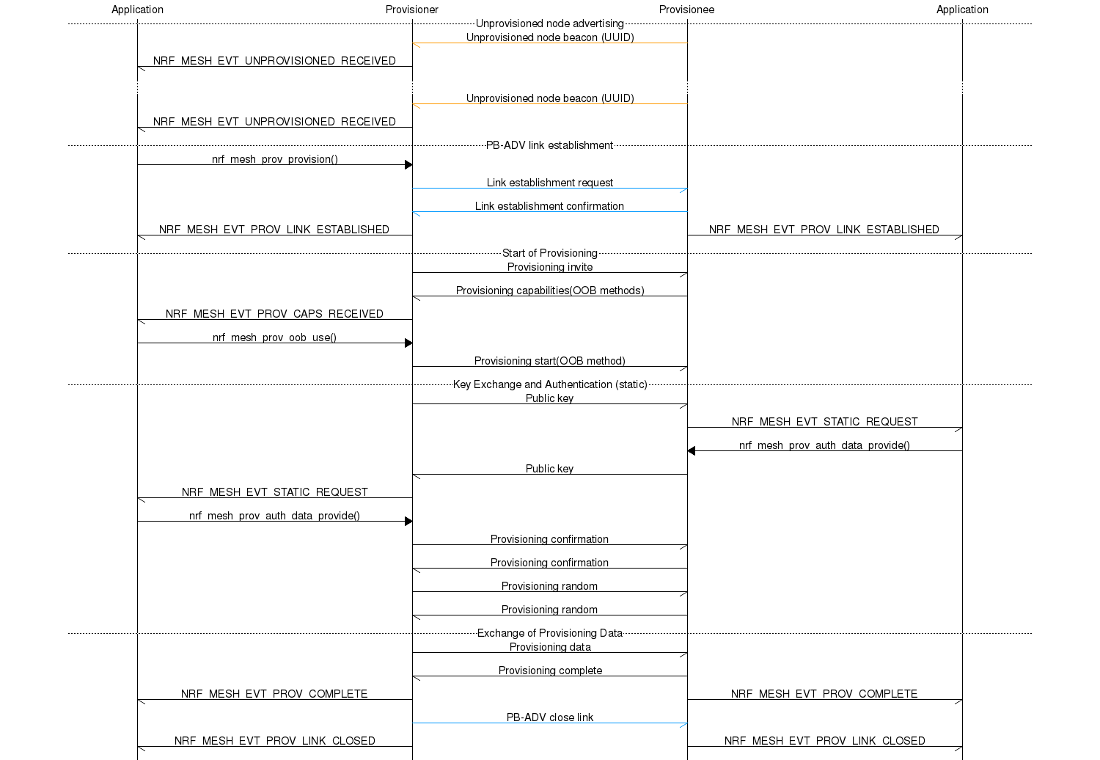
\includegraphics[scale=0.5]{images/provisioning.png}
            		\caption{Provisioning scenarios}
            	\end{center}
            \end{figure}

        \subsection{Thiết bị mới - Provisionee}
        Cách thức hoạt động của một thiết bị mới - unprovisioned hay provisionee: Tiến hành khởi tạo - bao gồm phát beacon để báo rằng mình cần tham gia provisioning, sau đó ở trạng thái chờ sự kiện. Khi bắt được sự kiện yêu cầu kết nối - lời mời provisioning từ provisioner thì đáp lại, tiếp đến chờ đáp lại các sự kiện xác thực, cuối cùng là kết thúc quá trình.
        \begin{figure}[h!]
        	\begin{center}
        		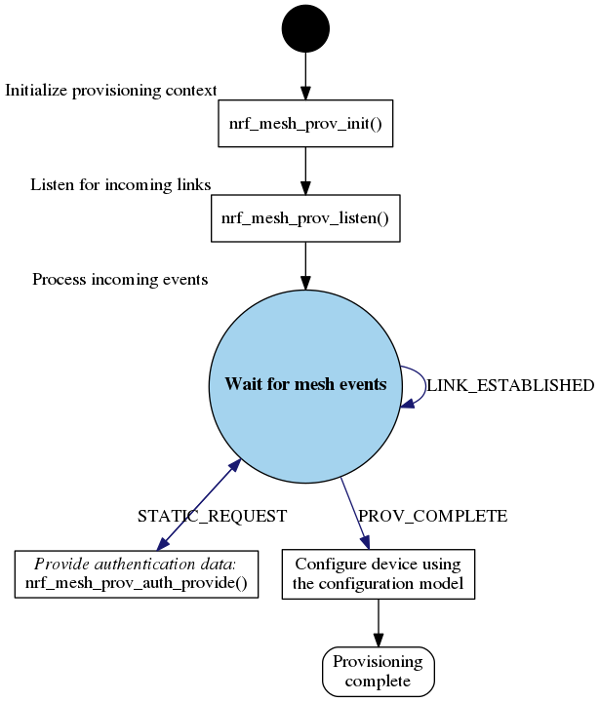
\includegraphics[scale=0.6]{images/provisionee_app_flowchart.png}
        		\caption{Provisionee flowchart}
        	\end{center}
        \end{figure}
	\newpage
        \subsection{Thiết bị Provisioner}
        Là thiết bị hoặc node chịu trách nhiệm thực hiện quá trình provisioning trong mạng mesh. Chúng thường là một phần của các thiết bị gateway - các thiết bị cung cấp một cầu nối giữa mạng mesh và các giao thức kết nối khác.  Cách thức hoạt động của một provisioner: sau các bước khởi tạo thì chờ beacon từ thiết bị mới (unprovisioned), sau đó mời tham gia quá trình provisioning. Trong bước xác thực, tùy theo đối tượng cần provisioning có hay không có hỗ trợ xác thực out-of-band (OOB) mà tiến hành xác thực theo cách tương ứng.
        \begin{figure}[h!]
        	\begin{center}
        		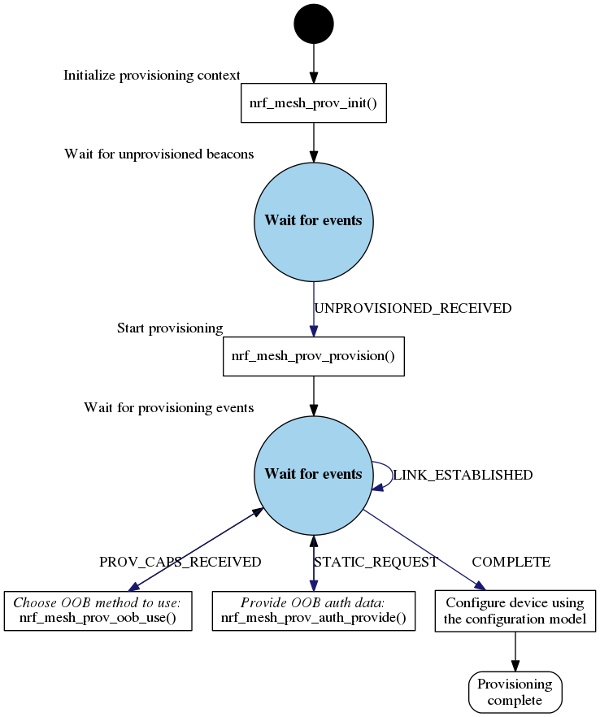
\includegraphics[scale=0.6]{images/provisioner_app_flowchart.png}
        		\caption{Provisioner flowchart}
        	\end{center}
        \end{figure}
        \subsection{Rời khỏi mạng} \label{removenode}
        Sau một thời gian hoạt động, việc phải loại bỏ một số node ra khỏi mạng là điều không thể tránh khỏi, có thể vì nhiều lý do như: node bị hỏng, chuyển node sang một khu vực khác với một mạng mesh khác, thay node mới,... Trong trường hợp nếu không có quy trình loại bỏ node, mạng sẽ đối mặt với nguy cơ bị tấn công kiểu Trashcan, kẻ tấn công có thể khai thác những node bị bỏ đi, lúc này chắc chắn lớp bảo vệ sẽ kém, để lấy thông tin và xâm nhập mạng. Bluetooth Mesh áp dụng 2 bước xử lý sau:
        \begin{itemize}
            \item Cho node bị loại bỏ vào danh sách đen.
            \item Tiến hành cấp lại NetKey cho các node trong mạng trừ node trong danh sách đen. 
        \end{itemize} 

        Quá trình này cần có một thời gian chuyển tiếp, trong thời gian này cả 2 key cũ và mới đều hợp lệ. Sở dĩ cần có thời gian chuyển tiếp này là vì các node low-power thỉnh thoảng mới hoạt động, do đó cần có thời gian để chúng nhận được chìa mới từ node friend của mình.
        \section{Khái niệm Friendship}
       Để có thể ở trong trạng thái sleep lâu dài, các node low power (LPNs) cần tiến hành thiết lập mối quan hệ Friendship với một node ``hàng xóm'' của mình, sau khi thiết lập xong thì node đó trở thành ``friend'' của LPN. Trước khi đi sâu hơn về khái niệm này, chúng ta cần làm quen với một vài tham số:
       \begin{itemize}
	\item ReceiveDelay: Khoảng thời gian từ lúc LPN gửi yêu cầu đến node friend cho đến lúc nó thức dậy lần nữa để bắt đầu nhận dữ liệu. Trong thời gian này LPN vẫn tiếp tục sleep, node friend thì tiến hành chuẩn bị dữ liệu để đáp lại yêu cầu đó.
	\item ReceiveWindow: Khoảng thời gian LPN thức dậy và lắng nghe, lúc này node friend mới có thể gửi dữ liệu cho LPN.
	\newpage
	\begin{figure}[h!]
        	\begin{center}
        		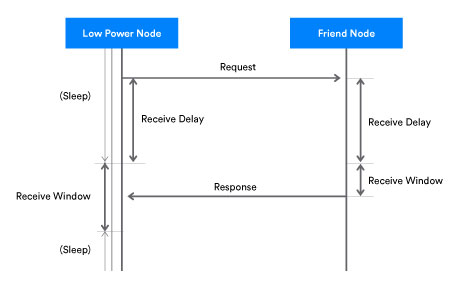
\includegraphics[scale=0.6]{images/friendship-1.jpg}
        		\caption{Hình mô tả ReceiveDelay và ReceiveWindow}
        	\end{center}
        	\end{figure}
        	\item PollTimeout: Khoảng thời gian tối đa giữa 2 lần LPN gửi yêu cầu cho node friend, nếu quá thời gian này mà vẫn không nhận được yêu cầu từ LPN, node friend sẽ kết thúc ``tình bạn'' với nó.
        	\begin{figure}[h!]
        	\begin{center}
        		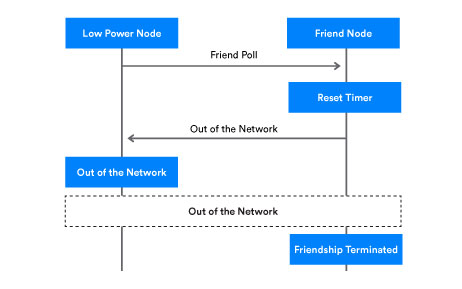
\includegraphics[scale=0.6]{images/friendship-2.jpg}
        		\caption{Hình mô tả PollTimeout}
        	\end{center}
          \end{figure}
       \end{itemize}
       \subsection{Các bước thiết lập Friendship}
       \begin{enumerate}
       \item Node LPN gửi ``yêu cầu kết bạn'', yêu cầu này sẽ không được relay vì nó chỉ có thể kết bạn với những node trong phạm vi kết nối của mình, ngoài ra các node trong phạm vi nhưng không hỗ trợ chức năng Friendship cũng sẽ bỏ qua yêu cầu này. Yêu cầu kết bạn này bao gồm cả 3 thông số ReceiveDelay, ReceiveWindow và PollTimeout.
       \item Node thỏa mãn các yêu cầu để trở thành Friend sẽ gửi lại Friend Offer cho LPN. Gói này bao gồm nhiều tham số như ReceiveWindow có thể hỗ trợ, sức chứa của buffer - buffer này để chứa ``hộ'' các dữ liệu được gửi tới LPN trong lúc nó ngủ và được gọi là Friend Queue,...      
       \item Khi LPN nhận được Friend Offer, nó sẽ dùng một thuật toán để chọn ra 1 Friend (nếu có nhiều Friend Offer), thuật toán này do người phát triển ứng dụng định nghĩa: có thể là ưu tiên node gần hơn hoặc node có khả năng hỗ trợ Friend Queue lớn hơn.
       \item Sau khi đã chọn được Friend, LPN gửi Friend Poll cho node đó.
       \item Sau khi nhận được Friend Poll, node Friend trả lời bằng Friend Update. Mối quan hệ Friendship chính thức được thiết lập.
       \end{enumerate}
       \subsection{Giao tiếp trong Friendship}
       Sau khi đã ``kết bạn'', LPN và node Friend của nó sẽ tiến hành giao tiếp theo các bước sau:
       \begin{figure}[h!]
        	\begin{center}
        		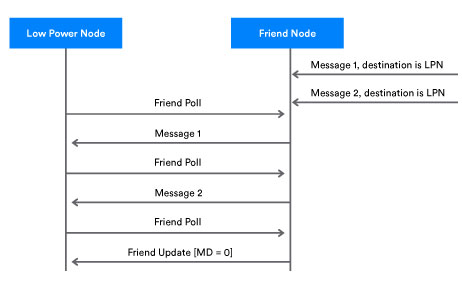
\includegraphics[scale=0.6]{images/friendship-3.jpg}
        		\caption{Hình mô tả quá trình giao tiếp}
        	\end{center}
          \end{figure}
       \begin{enumerate}
	\item Khi node Friend nhận được dữ liệu được gửi đến node LPN là ``bạn'' của nó, nó sẽ lưu vào Friend Queue. Trong hình trên, có thể thấy node Friend đã lưu lại Message 1 và Message 2 thay cho node LPN.
	\item Sau một chu kỳ ngủ, node LPN sẽ gửi yêu cầu Friend Poll đến cho node Friend của mình để kiểm tra có dữ liệu mới hay không.
	\item Nếu có dữ liệu mới, node Friend sẽ gửi ngược lại cho LPN, cứ mỗi lần LPN nhận được dữ liệu nó lại gửi thêm Friend Poll.
	\item Đến khi nào nhận được Friend Update (với tham số More Data = 0) nghĩa là không còn dữ liệu nữa, quá trình giao tiếp này sẽ kết thúc, LPN không gửi Friend Poll nữa.
      \end{enumerate}
      
      Các gói tin giữa node Friend và LPN đều được mã hóa bằng một loại key Friend và chỉ có 2 node này mới có khả năng đọc được.